% begin module limit-at-infinity-ex5
\begin{frame}
\begin{example} %[Example 6, p. 131]
\begin{columns}[c]
\column{.45\textwidth}
Evaluate $\lim_{x\to \infty} \sqrt{x^2+1}-x$.

\psset{xunit=0.7cm, yunit=0.7cm}
\begin{pspicture}(-5, -5)(5,5) 
\psframe*[linecolor=white](-5,-5)(6,5) 
\psaxes[ticks=none, labels=none]{<->}(0,0)(-2,-0.5)(6,4.5)
\psLabelXOne
\psLabelYOne
%Function formula: - (x)+sqrt{}((x)^{2}+1) 
\uncover<9->{
\psplot[linecolor=red, plotpoints=1000]{-1.95}{5.95}{1 x 2 exp add sqrt x -1 mul add }
\rput[lb](1,1){\footnotesize $y=\sqrt{x^2+1}-x$}
\psline[linecolor=blue](-1.95, 0)(5.95, 0)
}
\end{pspicture} 
%\ \only<handout:0| -8>{%
%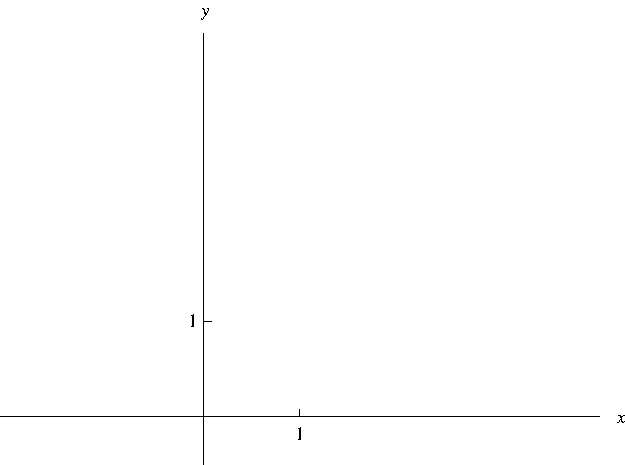
\includegraphics[width=5cm]{curve-sketching/pictures/04-04-ex5a.pdf}%
%}%
%\only<9->{%
%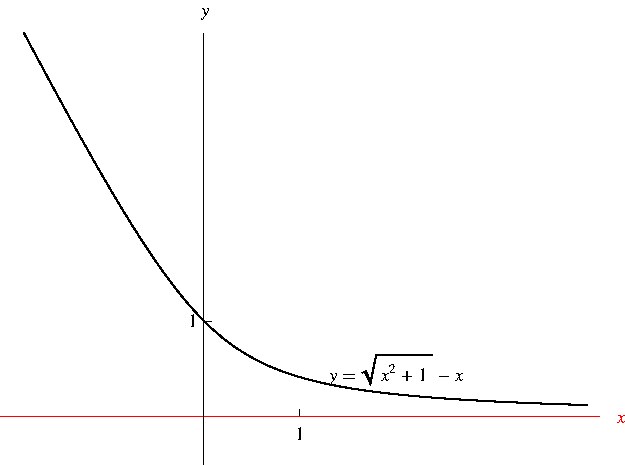
\includegraphics[width=5cm]{curve-sketching/pictures/04-04-ex5b.pdf}%
%}%
\begin{itemize}
\item<2->  $\sqrt{x^2+1}\to \infty$ and $x\to \infty$ as $x\to \infty$.
\item<2->  It isn't clear what happens to the difference.
\item<7-| alert@7>  Divide top \& bottom by $x$.
\end{itemize}
\column{.55\textwidth}
\begin{itemize}
\item<3-| alert@3-4>  Standard approach: multiply top and bottom by conjugate radical.
\end{itemize}
\abovedisplayskip=0pt
\belowdisplayskip=0pt
\begin{eqnarray*}
&&%
\uncover<2->{%
\lim_{x\to \infty} \left( \sqrt{x^2+1}-x\right) \uncover<4->{\alert<handout:0| 4>{\frac{\sqrt{x^2+1}+x}{\sqrt{x^2+1}+x}}}%
}%
\\%
&&%
\uncover<5->{%
 = \lim_{x\to \infty} \frac{(x^2+1)-x^2}{\sqrt{x^2+1}+x}%
}%
\\%
&&%
\uncover<6->{%
 = \lim_{x\to \infty} \frac{1}{\sqrt{x^2+1}+x}\uncover<7->{\alert<handout:0| 7>{\cdot \frac{\frac{1}{x}}{\frac{1}{x}}}}%
}%
\\%
&&%
\uncover<8->{%
 = \lim_{x\to \infty} \frac{\frac{1}{x}}{\sqrt{1+\frac{1}{x^2}}+1}%
}%
\\%
&&%
\uncover<9->{%
 = \frac{0}{\sqrt{1+0}+1} = 0%
}%
\end{eqnarray*}
\end{columns}
\end{example}
\end{frame}
% end module limit-at-infinity-ex5
